\clearpage %poner esta linea al inicio de cada capitulo
\chapter{Dise\~no de la m\'aquina}

\section{Diseño Mecánico}\label{mecanico}

Para la implementación de la v-made, se tuvo en cuenta en primera medida la distribución propuesta en la sección \ref{planteamiento},teniendo en cuenta esto, la representación gráfica del diseño planteado se expone en la \autoref{fig:hibrida} : 


\begin{figure}[H]
    \centering
    \resizebox*{12 cm}{!}{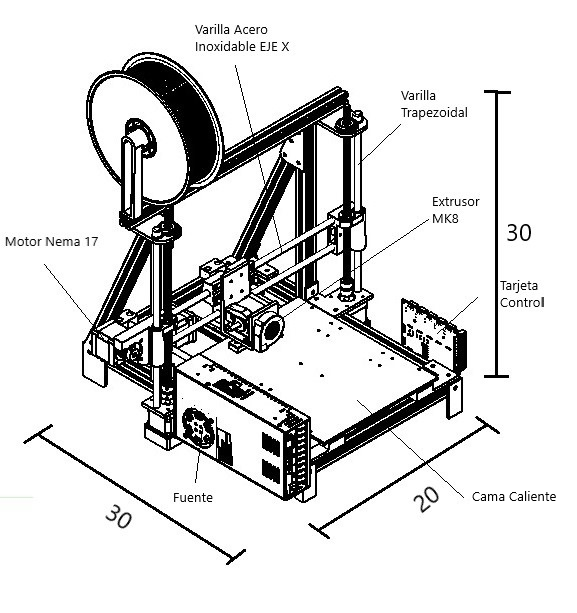
\includegraphics{Figs/maquina.png}}
    \caption{Plano general V-made}
    \label{fig:hibrida}
\end{figure}

Conociendo la distribución y los elementos que componen la V-MADE,se da desarrollo al diseño mecánico, esto teniendo en cuenta la trayectoria máxima restringida por su área y la distribución planteada en la misma. \\

Como primera medida es de vital importancia conocer los esfuerzo involucrados en el funcionamiento de la maquina,ya que esto determina que materiales son los indicados para su construcción y cual sera la resistencia real de la maquina.Por lo cual se realizan cálculos de flexión en los ejes X y Y. Se toman estos ejes ya que están sometidos a tensión, y el objetivo es encontrar un diámetro que garantice  el soporte de las piezas presentando una mínima flexión, lo que supondrá una mayor resistencia de la máquina.\\

\subsection{Eje X}

\begin{figure}[H]
    \centering
    \resizebox*{8cm}{!}{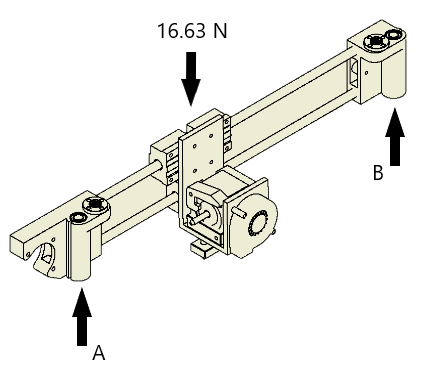
\includegraphics{Figs/EJEX.PNG}}
    \caption{Eje X.}
    \label{fig:preuba1}
\end{figure}

Datos de masas involucradas:

\[m_{extrusor}=480\text{g}\]
\[m_{soporte}=100\text{g}\]
\[m_{varillas}=550\text{g}\]
\[m_{acoples}=260\text{g}\]

\begin{equation}
m_{total}=1390\text{g}
\label{eq:101}
\end{equation}

Con la masa total, encontramos la fuerza aplicada en el eje

\begin{equation}
F_x=1390\times9.81=13.63\text{N}
\label{eq:102}
\end{equation}

Al obtener la fuerza aplicada en el eje x, se realiza un cálculo de Momento flector y Fuerza cortante, esto con el fin de obtener los datos de los esfuerzos a los que esta sometido el eje con una carga puntual. A partir de los resultados, se compara con la distribución de la fuerza y se determinar de manera idonea el material a usar en la construcción del eje.\\


\begin{figure}[H]
    \centering
    \resizebox*{11cm}{!}{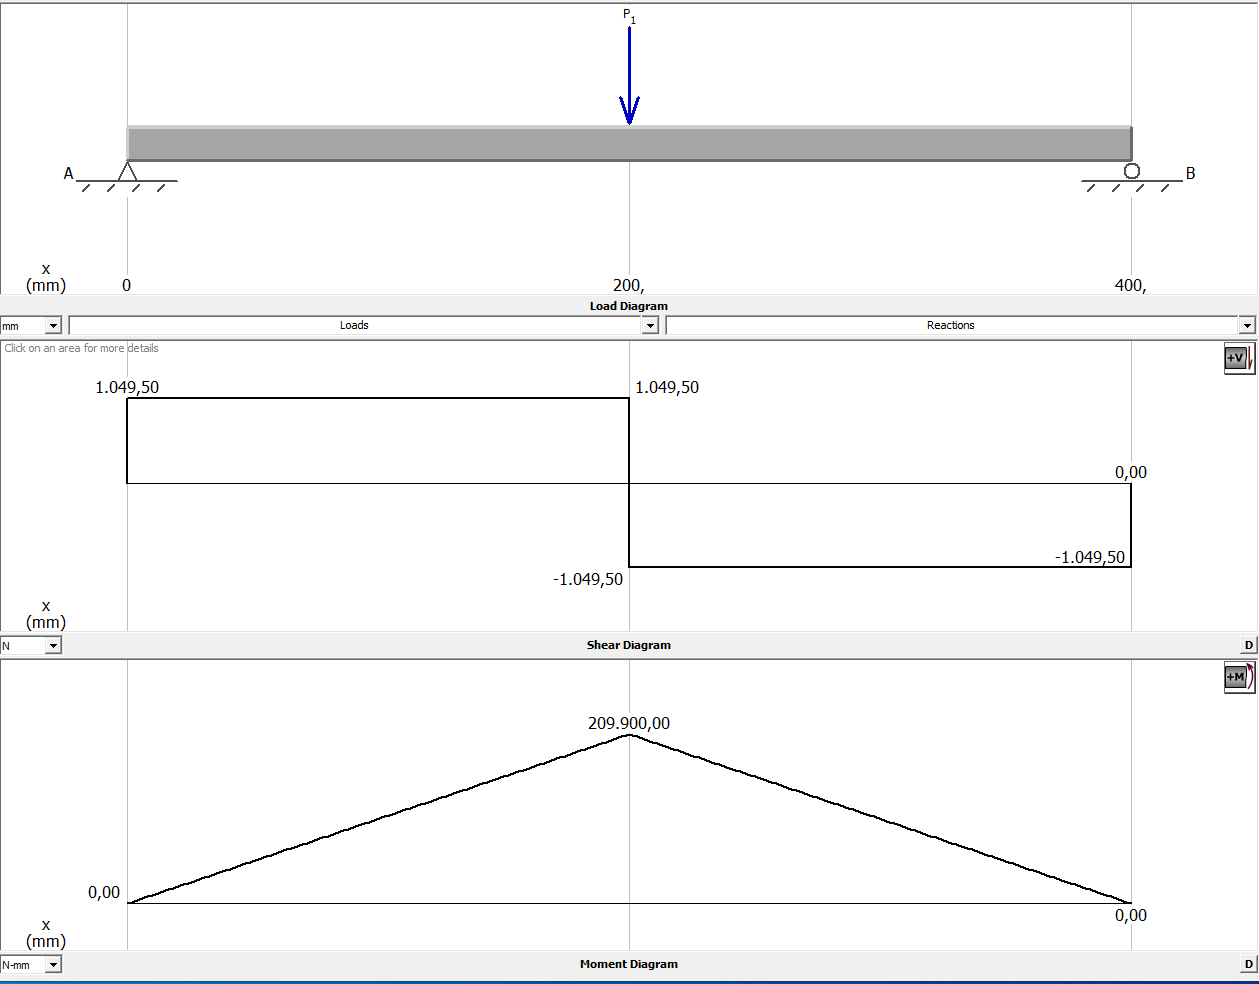
\includegraphics{Figs/EJEXDG.PNG}}
    \caption{Momento Flector y Fuerza Cortante Eje X.}
    \label{fig:CAL1}
     \textbf{Fuente: MDSolids}
\end{figure}

Se determinan que la fuerza se distribuye en dos ya que el eje esta construido a partir de dos guías 

\[F_{xguia}=\frac{13.63}{2}=6.815\text{N}\]

Se toma como consideración, que la varilla está sometida a una carga puntual, por lo tanto el momento flector se puede expresar como en la \autoref{eq:103}.

\begin{equation}
M_{fx}=\frac{F_{xguia}L}{4}
\label{eq:103}
\end{equation}

\[M_{fx}=\frac{(6.815)(400)}{4}=681.5\text{N}\times \text{mm}\]

El esfuerzo debido al momento flector sera

\[\sigma_x=\frac{Mc}{I}=\frac{32M}{\pi d^3}\]

de la fórmula de máximo esfuerzo cortante
\begin{equation}
(\sigma_1-\sigma_2)\leq \frac{S_y}{n}   
\label{eq:104}
\end{equation}


calculando los esfuerzos principales

\[\sigma_m=\frac{\sigma_x+\sigma_y}{2}=\frac{16M}{\pi d^3}\]
\[\tau=\sqrt{(\frac{\sigma_x+\sigma_y}{2})^2+\tau_{max}^2}=\frac{16M}{\pi d^3}\]
Tomando los esfuerzos principales
\[\sigma_1=\tau_{max}+\sigma_m=\frac{32M}{\pi d^3}\]
\[\sigma_2=\tau_{max}-\sigma_m=0\]

Remplazando la \autoref{eq:104}

\[\frac{32M}{\pi d^3}\leq \frac{S_y}{n}\]

Despejando el diámetro

\begin{equation}
  d\geq (\frac{32Mn}{\pi S_y})^{\frac{1}{3}} 
  \label{eq:105}
\end{equation}

Resolviendo la \autoref{eq:105}, se obtiene el diámetro requerido para las cargas aplicadas en el eje.Se toma un factor de seguridad de 3 ya que las fuerzas son dinámicas durante el proceso, de esta manera se brinda la resistencia de la estructura.

\[d\geq (\frac{32(681.5)(3)}{\pi(235)})^{\frac{1}{3}} \]
\[d\geq 4.45\text{mm}\]


\subsection{Eje Y}


\begin{figure}[H]
    \centering
    \resizebox*{7cm}{!}{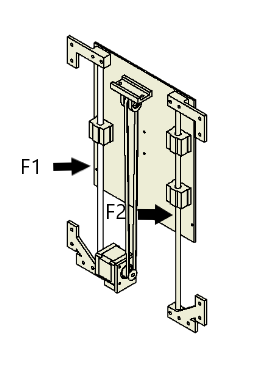
\includegraphics{Figs/EJEY.PNG}}
    \caption{Eje Y.}
    \label{fig:Y}
\end{figure}



Datos de masas involucradas:

\[m_{Cama}=600\text{g}\]
\[m_{soportes}=250\text{g}\]
\[m_{varillas}=550\text{g}\]
\[m_{SistemaPolea}=150\text{g}\]
\[m_{Motor}=350\text{g}\]

\begin{equation}
m_{total}=1900\text{g}
\label{eq:105}
\end{equation}

Con la masa total, encontramos la fuerza aplicada en el eje

\begin{equation}
F_y=1900\times9.81=18.63\text{N}
\label{eq:102}
\end{equation}

Se involucran las masas anteriormente descritas más las impresiones que se realicen,lo cual dependerá del tamaño de la pieza y el relleno. Para aproximar correctamente los esfuerzo involucrados, se toma como una fuerza distribuida a lo largo del eje como primera instancia. Seguido de calculos matematicos suponiendos dos cargas distribuidas por la distribvuión de los ejes.\\

\begin{figure}[H]
    \centering
    \resizebox*{14cm}{!}{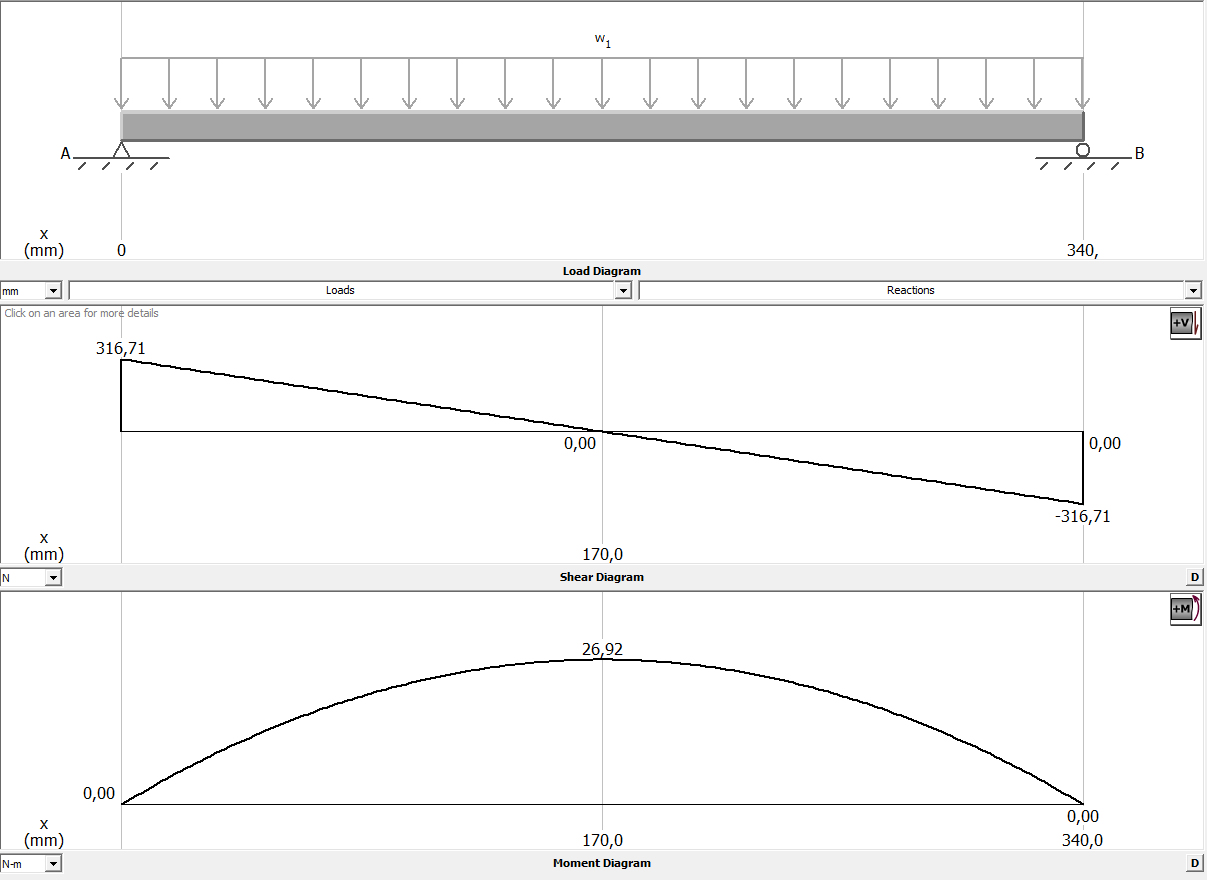
\includegraphics{Figs/ejeydg.PNG}}
    \caption{Momento Flector y Fuerza Cortante Eje Y.}
    \label{fig:CAL2}
     \textbf{Fuente: MDSolids}
\end{figure}

Como el eje esta construido a partir de dos guías,la fuerza se distribuye en dos para poder realizar un cálculo mas sencillo.

\[F_{xguia}=\frac{18.63}{2}=9.315\text{N}\]

Se toma como consideración, que la varilla está sometida a una carga puntual, por lo tanto el momento flector se puede expresar como en la \autoref{eq:103}.

\begin{equation}
M_{fy}=\frac{F_{yguia}L}{4}
\label{eq:103}
\end{equation}

\[M_{fx}=\frac{(9.315)(340)}{4}=791.775\text{N}\times \text{mm}\]

El esfuerzo debido al momento flector sera

\[\sigma_x=\frac{Mc}{I}=\frac{32M}{\pi d^3}\]

de la fórmula de máximo esfuerzo cortante
\begin{equation}
(\sigma_1-\sigma_2)\leq \frac{S_y}{n}   
\label{eq:104}
\end{equation}


calculando los esfuerzos principales

\[\sigma_m=\frac{\sigma_x+\sigma_y}{2}=\frac{16M}{\pi d^3}\]
\[\tau=\sqrt{(\frac{\sigma_x+\sigma_y}{2})^2+\tau_{max}^2}=\frac{16M}{\pi d^3}\]
Tomando los esfuerzos principales
\[\sigma_1=\tau_{max}+\sigma_m=\frac{32M}{\pi d^3}\]
\[\sigma_2=\tau_{max}-\sigma_m=0\]

Remplazando la \autoref{eq:104}

\[\frac{32M}{\pi d^3}\leq \frac{S_y}{n}\]

Despejando el diámetro
\[d\geq (\frac{32Mn}{\pi S_y})^{\frac{1}{3}}\]

Aplicando la formula se obtiene

\[d\geq (\frac{32(791.775)(3)}{\pi(235)})^{\frac{1}{3}} \]
\[d\geq 4.7 \text{mm}\]

Obteniendo los resultados de diámetro requerido y a partir de los análisis presentados en las \autoref{fig:CAL1} y \autoref{fig:CAL2}, realizadas para cada uno de los casos a tensión. Se procede a buscar el material adecuado para la construcción de los ejes. 

\begin{table}[H]
\begin{center}
\begin{tabular}{ p{1.5cm} p{2.5cm} p{2.5cm} p{2cm} p{2cm} p{1cm} p{3cm}}
\toprule[0.6mm]
Acero Inoxidable & Resistencia a la tracción(MPa) & Esfuerzo de Fluencia(MPa)& Elongación en 50mm(\%) & Reduccion de area(\%) & Dureza & Condiciones\\
\midrule
\multirow{3}{2cm}{304} & 585 & 235& 60 &70& 149& Barra Recocida  \\ 
\cmidrule{2-7}
& 690 & 415 &45& &212& Recocido y estirado en frió \\ 
\cmidrule{2-7}
& 860 & 655& 25 && 275& Estirada en frió de alta resistencia \\ 
\bottomrule[0.6mm]
\end{tabular}
\caption{Propiedades Mecánicas Acero Inoxidable.}
\textbf{Fuente:\citep{acero} }
\label{tabla:acero}
\end{center}
\end{table}




\begin{table}[H]
\begin{center}
\begin{tabular}{l c c c}
\multicolumn{2}{c}{\textbf{Acero Inoxidable 304}} \\
\toprule[0.6mm]
Densidad& $7.93 \text{g}/ \text{cm}^3$  \\ 
Punto de Fusión& $1398-1454\: C^{\circ}$ \\ 
Calor Especifico & $500\frac{J}{(Kg*K)} a \:20\: C^{\circ}$ \\ 
Resistividad Eléctrica & $0.73\mu \Omega \times \text{m}$ \\ 
Permeabilidad Magnética & 1.02  \\ 
Modulo Elástico & 193 GPa   \\
Difusividad Térmica & $3.84 \text{mm}^2/\text{s}$  \\ 
\midrule
\multirow{2}{5cm}{Coeficiente de conductividad Térmica}& 16.3 (100 $C^{\circ}$)  \\ 
&21.5 (500 $C^{\circ}$)\\
\midrule
\multirow{3}{3cm}{Coeficiente de dilatación lineal}& 17.2(0-100 $C^{\circ}$)\\ 
& 17.8 (0-300 $C^{\circ}$)\\ 
&18.4 (0-500 $C^{\circ}$)\\ 
\bottomrule[0.6mm]
\end{tabular}
\caption{Propiedades Físicas.}
\textbf{Fuente:\citep{acero} }
\label{tabla:Fisicas}
\end{center}
\end{table}



A partir de los datos de la \autoref{tabla:acero} y \autoref{tabla:Fisicas},se selecciona el acero inoxidable 304 barra recocida, como soporte de los ejes con un diámetro de 8 mm, se toma como base los datos técnicos del material, en lo que demuestra su resistencia a las deformaciones por cargas y cambios de temperatura.\\ 


\subsection{Soporte del Extrusor } 

\begin{figure}[H]
    \centering
    \resizebox*{10cm}{!}{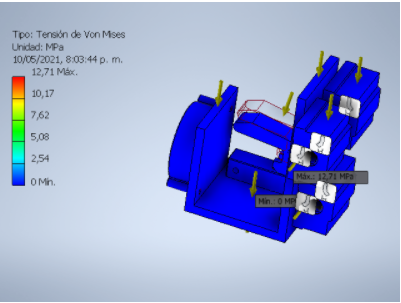
\includegraphics{Figs/extrusor1.PNG}}
    \caption{Simulación Von Mises }
    \label{fig:sim}
\end{figure}

$Peso =0.1 KG$\\
$Longitud=0.09 m$\\

Se calcula el momento flector a través de la fuerza que produce este soporte por su distancia

\[M_{soporte}=F_s\times longitud\]
\[M_{soporte}=(0.981)(0.09)\]
\[M_{soporte}=0.088 \text{N}\]

Con el resultado obtenido, podemos calcular el esfuerzo de diseño máximo.
\[\sigma'<\sigma_d=\frac{S_y}{N}\]

Operando
\[\sigma_d=\frac{27.76}{2}\]
\[\sigma_d=13.88\text{MPa}\]


COMPARAR CON LA SIMULACIÓN QUE SE VA A COLOCAR COMO IMAGEN

\subsection{Cortante en el soporte en x}\\

\begin{figure}[H]
    \centering
    \resizebox*{6cm}{!}{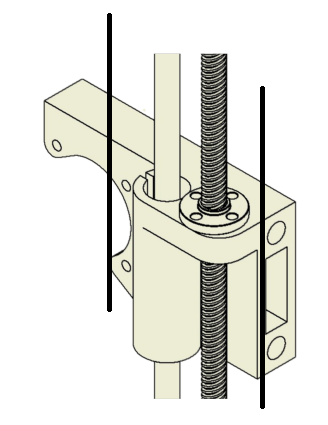
\includegraphics{buje.png}}
    \caption{Cortante soporte}
    \label{fig:cortante}
\end{figure}



\textbf{Momento Inercia}
\vspace{5mm}
\[I=\frac{1}{12}B^3h\]
\[I=\frac{1}{12}(0.02)^3(0.02)\]
\[F=1.33\times 10^{-8} \]

\[F=\frac{3\text{kg}}{2}(9.8)=14.71\text{N}*0.001=0.01471\]
\[\sigma_{Max} =\frac{M_c}{I}\]
\[\sigma_{Max}=\frac{0.01471(1.5)}{1.33\times10^{-8}}=1.659\text{MPa}\]

\textbf{Esfuerzo cortante}\\

\[\sigma_{Max} =\frac{3V_c}{2A}\]
\[A=\frac{\pi\times0.08^2}{4}=5.026\text{m$^2$}\]
\[\sigma_{Max}=\frac{3(14.71)}{3(5.026)}=0.39023\:\text{MPa}=390\:\text{KPa}\]

\subsection{Diseño del sistema de transmisión}

El diseño de transmisión se realiza a través de un sistema polea-correa la fuerza para mover este sistema está determinada por la siguiente ecuación

\begin{equation}
F=F_n(\frac{v^2}{2D_pg}+f_r)
\label{eq:106}
\end{equation}

Donde $F_n$ es la fuerza normal total en todo el eje , v la velocidad de impresión que se está usando, $D_p$ es la distancia entre poleas y $f_r$ es la fuerza de rozamiento de acero con acero que es de 0,18.Con esta información se determina la fuerza de la polea en cada uno de los ejes.

\[F_{ejex}=13.63(\frac{0.06^2}{(2)(0.4)(9.81)}+0.18)=2.45 \text{N}\]

\[F_{ejey}=18.63(\frac{v^2}{(2)(0.34)(9.81)}+0.18)=3.36 \text{N}\]

\subsection{Cálculo en el eje coordenado z}

Teniendo en cuenta los esfuerzos que se generan en cada uno de los ejes,se procede a realizar un cálculo del torque necesario para el desplazamiento del mecanismo,para su desarrollo es indispensable tener en cuenta la inercia que se produce en conjunto y la fuerza de fricción a vencer, con la solución de estos datos se puede proceder a determinar cuales son los motores indicados para esta aplicación.

\begin{figure}[H]
    \centering
    \resizebox*{8cm}{!}{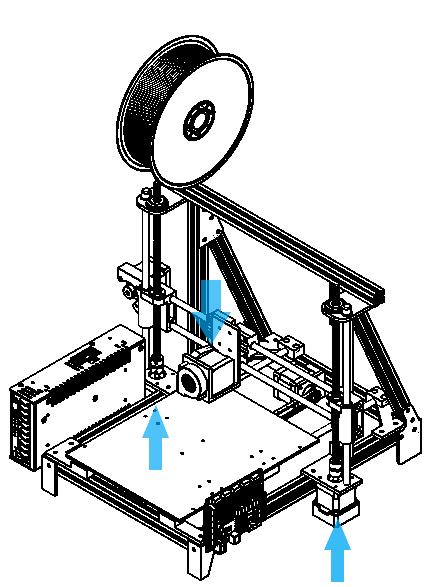
\includegraphics{Figs/EJE_Z.png}}
    \caption{Eje z}
    \label{fig:eje z}
\end{figure}

\textbf{Torque Requerido Para Mover el Sistema}

Para obtener este dato es necesario realizar el cálculo de inercia en el sistema, por lo cual tenemos como datos generales

\begin{itemize}
	\item $Peso Movimiento=4Kg=8.81 Libras$
	\item $Paso Tornillo=2 mm$
\end{itemize}

Conversión paso mm a hilos por pulgada

\[P=(\frac{2}{25.4})=0.078\]
\[0.078=\frac{1}{N}\]
\[N=12.82\]

\textbf{Inercia Plataforma}

\begin{equation}
Ip=(\frac{W}{P^2})(\frac{1}{2\pi })^2
\label{eq:11}
\end{equation}

\[I_p=(\frac{8.81}{(12.82)^2})\times0.025=0.0664 lb\times in^2\]

\textbf{Inercia Tornillo}

\begin{equation}
I_T=\frac{D^4L}{36}
\label{eq:12}
\end{equation}


$Diametro Tornillo= 8mm=0.3149 in$\\
$Longitud Tornillo= 400mm=15.74 in$\\

Con lo cual remplazamos la \autoref{eq:12}

\[I_t=\frac{(0.3149)^4(15.74)}{36}=4.2992\times10^{-3} lb\times in^3\]

\textbf{Total Inercia }

A partir de las inercias calculadas en el sistema, se realiza un promedio para encontrar el equivalente de inercia en la maquina.
\[I_{eq}=0.0664+4.2992\times 10^{-3}+0.2=0.27169 lb\times in^3\]

Obteniendo estos resultados es posible realizar el planteamiento del Torque requerido el cual esta dado por:


\begin{equation}
T_a=2\times I_{eq}\times\frac{w}{t}\times\frac{\pi \theta }{180}\times\frac{1}{24}
\label{eq:13}
\end{equation}

Donde

\begin{equation}
W=sps
\label{eq:13}
\end{equation}

$V_{max}=9000mm/min=(354.33in/min)$\\
$spr=240;$\\
$p=Paso tornillo=2mm=(12.82in)$\\

\begin{equation}
sps=\frac{V_l_m_a_x\times spr}{60}
\label{eq:13}
\end{equation}

\begin{equation}
sps=\frac{354.33\times240\times12.82}{60}=18170.04
\label{eq:13}
\end{equation}

\begin{equation}
T_a=2\times0.27169\times\frac{18170.04}{0.12}\times\frac{\pi\times1.5}{180}\times\frac{1}{24}
\label{eq:13}
\end{equation}

\[T_a=89.75\: oz\times in =0.63377427\: N\times m\]

A partir de las varillas roscadas se permite la movilización del eje Z y Y . Se debe presentar un avance lineal mínimo de 20 micrómetros para cumplir la resolución en la impresión de piezas.\\

\textbf{Torque requerido para vencer la fuerza de fricción}

\begin{figure}[H]
 \centering
  {
    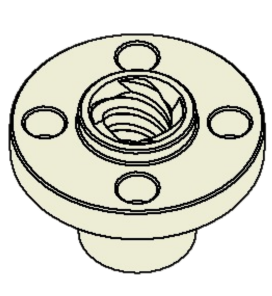
\includegraphics[width=0.25\textwidth]{ejez.png}}
  {
    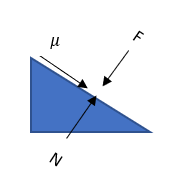
\includegraphics[width=0.3\textwidth]{TRI_CALCULOS.PNG}
    }
 \caption{Cortante Buje en z}
 \label{f:animales}
\end{figure}


Teniendo el dato del torque requerido para desplazar el sistema, es indispensable encontrar el valor para vencer la fuerza de fricción, ya que ha partir de estos datos, se tiene plena seguridad de que el sistema tendrá el torque necesario en cada uno de sus motores para el correcto desplazamiento del sistema.\\

$F_f=0.375lb$\\
$e_f_f=90 \% $\\

\begin{equation}
T_b=\frac{16\times F_f}{2\times\pi\timesp\times e_f_f}
\label{eq:13}
\end{equation}

\[T_b=1.0610\: lb\times in= 0,11987690392266312  N\times m\]

Obteniendo los datos de los torques, se procede a calcular cual seria el torque necesario por cada motor para dar un correcto desplazamiento en el proceso de manufactura con lo cual tenemos:

\textbf{Torque necesario}\\

\begin{equation}
T_R=\frac{(F*D_m)}{2}*\frac{L+π\mu*d_m}{\pi d_m -\mu*L}
\label{eq:201}
\end{equation}
\begin{equation}
T_R=\frac{34.33*6.858}{2}*\frac{2+\pi*0.17*6.858}{\pi*6.85-0.17*2}
\label{eq:200}
\end{equation}

\begin{equation}
T_R=24.52 N=0.2452Nm
\label{eq:202}
\end{equation}

\textbf{Área Trabajo Efectiva}\\

La capacidad de impresión es de 20$\times$25 se decidió tener solo esta área en cuenta, por limitaciones mecánicas en la distribución de los finales de carrera como se muestra en la \autoref{}, además basándonos en las pruebas que se muestran en el apartado de la  \autoref{fotos}, la distribución de la temperatura uniforme solo llegas hasta las medidas expuestas con anterioridad, delimitando el área efectiva no se tendrán problemas por delaminación o poca adherencia a la cama.\\


COLOCAR EL VOLUMEN EFECTIVO DE LA MAQUINA Y CUAL ES SU CONSUMO EN WATTS DE ESTA MANERA SE PUEDEN DEDUCIR COSTOS DE PRODUCCIÓN .



COLOCAR PESO DE LA MAQUINA Y UNCA IMAGEN QUE MUESTRE DONDE ESTAS LOS FINALES DE CARRERA Y REFERECIARLA


\section{Diseño de Control}\label{Dicontrol}

\textbf{Motores}

Para el control del movimiento y rapidez de los motores se envían pulsos (desplazamiento) a diferentes frecuencias (velocidad) a la tarjeta de micropasos. Los pulsos se envían por medio de señales PWM con periodo de trabajo del 50 \% a frecuencias que varían dependiendo de la velocidad requerida.\\

Los pasos se determinan mediante la resolución que tenga el motor.Para el caso del Nema 17 tiene una resolución de
1.8 grados,con lo que se aplica la \autoref{eq:108}

\begin{equation}
Pasos_{rev}=\frac{360}{1.8}=200 
    \label{eq:108}
\end{equation}
Esto significa que el motor opera a 200 paso completo, con lo cual se procede a calcular los micropasos

\begin{equation}
Pasos_{rev\frac{1}{16}}=\frac{360}{1.8/1.6}=3200 
    \label{eq:109}
\end{equation}

Para realiza el control en el dispositivo, de los motores respectivos en cada eje, se realiza el cálculo de pasos por milímetros mediante la \autoref{eq:110}


\begin{equation}
Pasos_{mm}=\frac{Paso_{motor}\times Micropasos Driver}{Paso_{correa}\times NumeroDientesPolea} 
    \label{eq:110}
\end{equation}

Donde los pasos por revolución del motor son 200, los Micropasos del driver son 32 , el Paso de la correa es 2[mm] y el Número de dientes de la polea es 20 .

\[Pasos_{mm}=\frac{200\times 32}{2\times 20}=160 \]

Para el eje z es necesario tener en cuenta el tornillo y su acople por lo tanto

\begin{equation}
Pasos_{mm}=\frac{Paso_{motor}\times Micropasos Driver}{PasoRoscaTornillo} 
    \label{eq:111}
\end{equation}

Donde el paso de la rosca del tornillo es de 2 mm 

\[Pasos_{mm}=\frac{200\times 32}{2}=3200 \]

Para el extrusor se cálcula

\begin{equation}
Pasos_{mm}=\frac{Paso_{motor}\times Micropasos Driver}{DiametroEfectivoEngranaje\times \pi} 
    \label{eq:112}
\end{equation}

El diámetro efectivo del engranaje es 10.95 mm

\[Pasos_{mm}=\frac{200\times 32}{10.95 mm \times \pi}=186.1547\]

Estos resultados se implementaron en el código y mostraron buenos resultados a la hora de imprimir, es necesario destacar que se seleccionaron aceleraciones mas bajas a las estándar, para obtener mejor estabilidad y pocas vibraciones, En el motor del extrusor se realizo lo contrario, ya que al aumentar su aceleración se produce menor desperdicio de material en la construcción de modelos.\\

\textbf{Temperatura}

El control que se realizo para extrusor y cama están basados en las características de los dispositivos seleccionados en la \autoref{selector}.Esto conlleva a que en la programación implementada en Marlin, se seleccione en dispositivo de control el numero 5, que hace referencia a una termoculpa TP100, este dispositivo permite la adquisición de datos de temperatura,logrando así el desarrollo de control para la cama caliente. Se coloco una prueba de seguridad en este apartado, para saber si algún termistor se encuentra dañado, esto se desarrollo por medio de definir un rango de  temperaturas que va desde 5-150 en la cama y en el extrusor de 5-275 ,si este rango es menor al enceder la maquina, se puede concluir que esta dañado algún termistor. \\

El control se desarrollo con un código que sintoniza un PID automáticamente, contando la cantidad de ciclos que quiere, índice de temperatura y la temperatura objetivo. Con estos datos el código, realiza iteraciones basado en unos valores preestablecidos, en el que su rango es muy cercano a los valores objetivos, de esta manera se obtiene un buen desarrollo de control lo que genero como resultados.\\



\begin{table}[H]
\begin{center}
\begin{tabular}{ c c c}
\multicolumn{3}{c}{\textbf{Extrusor}} \\
\toprule[0.6mm]
K_P & K_I & K_D\\
\midrule
19.82 & 1.60 & 61.45 \\ 
\bottomrule[0.6mm]
\end{tabular}
\caption{Constantes PID extrusor.}
\label{tabla:extrusor}
\end{center}
\end{table}

\begin{table}[H]
\begin{center}
\begin{tabular}{ c c c}
\multicolumn{3}{c}{\textbf{Cama}} \\
\toprule[0.6mm]
K_P & K_I & K_D\\
\midrule
97.1 & 1.4 & 1675.16 \\ 
\bottomrule[0.6mm]
\end{tabular}
\caption{Constantes PID cama.}
\label{tabla:cama}
\end{center}
\end{table}

COLOCAR LA GRÁFICA DEL CONTROL Y UNA COMPARCION CON LA UNA IMPLEMENTACIÓN PROPIA CON FUNCIÓN DE TRANSFERENCIA


\textbf{Finales de carrera}

Se aplica un control on/off donde los sensores indican la posición limite en cada uno de los ejes,mandando uno o cero lógico al sistema, la lógica en el Marlin, se desarrollo teniendo en cuenta la posición en la que se encuentran los finales de carrera, en la que se determino que se active el control en la posición mínima y que los motores vayan desde el otro extremo hacia el final de carrera para su posterior activación.  \\

\textbf{Sistema Informático}

Como primera medida en la programación general de Marlin, es necesario seleccionar el tipo de tarjeta que esta implementada, en este caso 0,esto con el objetivo de tener una identificación correcta de los pines de la familia de la tarjeta en la programación.Para la deposición de material, se programa únicamente un extrusor pero se deja la posibilidad para activar dos dentro del programa, los ventiladores de la maquina se dejan activos desde el momento que se enciende la maquina hasta que se apaga,esto se realiza para que no se tengan altas temperaturas en los dispositivos. \\

Otra configuración que cabe destacar, son los baudios que se seleccionaron ya que este dato es el número de unidades de señal por segundo que trasmite la impresora hacia su receptor, es necesario recordar que el valor que se coloco en la configuración, es indispensable colocarla en el programa que genera el gcode ya que de lo contrario no se realizara la impresión.\\

COLOCAR ANEXOS QUE MUESTREN EL CÓDIGO DE PROGRAMACIÓN CORRESPONDIENTE Y ACA DAR UNA EXPLICACIÓN DE LA ESTRUCTURA QUE SE UTILIZO\\


\textbf{Modulo de Comunicación}

Se toma la decisión del uso de este dispositivo frente a un modulo Wifi ya que dentro de sus prestaciones brinda más control sobre la configuración de su impresora 3D , teniendo muy pocas limitaciones y lo ayuda a producir impresiones 3D de mayor calidad sin tantos problemas de comunicación.\\

COMPLEMENTAR EL MODULO DE CO0MUNICACION QUE ES LA RASPBERRY

\section{Etapas del Proceso}

Las etapas del proceso que se necesitan realizar, para un correcto funcionamiento de la V-MADE, se exponen en el esquema de la \autoref{fig:diagrama}, esta representación da una explicación de los pasos necesarios desde el inicio de diseño hasta la construcción de la pieza.

\begin{figure}[H]
    \centering
    \resizebox*{9 cm}{!}{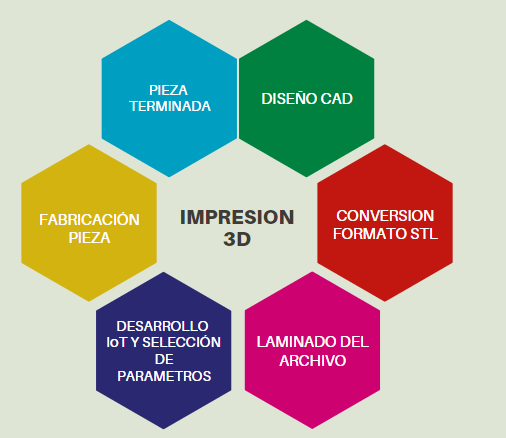
\includegraphics{Figs/PROCESO.PNG}}
    \caption{Etapa Proceso}
    \label{fig:diagrama}
\end{figure}

\textbf{DISEÑO CAD}: A partir de alguno de los paquetes de diseño existentes, se realiza un proceso de modelado de la pieza, incluyendo análisis de propiedades física y resistencia. Lo que proporcionara un gran apoyo en la construcción del objeto.  \\

\textbf{CONVERSIÓN FORMATO STL}: “Con la intención de unificar y simplificar el proceso se opta por emplear un formato común llamado STL. Este formato de archivo excluye información como color, texturas y propiedades físicas las cuales no son necesarias en la impresión 3D. Como resultado de este proceso se obtiene un archivo STL de la misma pieza esta vez formada por triángulos como aproximación al objeto CAD.''\citep{sainz}\\

\textbf{LAMINADO }:“ En este proceso se prepara el archivo STL para ser fabricado. Se ajusta el tamaño y la disposición y orientación del objeto sobre la superficie de impresión. Este software ejecuta un proceso sobre el
objeto STL demoniado laminado el cual crea capas de un grosor determinado según proceda. Este programa también es capaz de crear estructura auxiliar para soportar el objeto durante la impresión.''\citep{sainz}\\

\textbf{DESARROLLO IoT y SELECCIÓN DE PARÁMETROS}:Se logra visualizar el proceso de la impresión,a través de la interoperabilidad que brinda Octoprint, Además de la posibilidad de seleccionar la resolución que se desea manejar, el relleno y otros parámetros para proporcionar un buen resultado final .\\

\textbf{FABRICACIÓN PIEZA}:Construcción de la pieza capa por capa a través del control numérico implementado en la V-MADE \\
\textbf{PIEZA TERMINADA}:Solido que representa el diseño propuesto al inicio del proceso de Impresión.\\

\section{Selección de los dispositivos electrónicos} \label{selector}

\textbf{Motores}

Para determinar cual es el motor que mejor se desempeñaría , se realizo una búsqueda de distintos motores y sus aplicaciones más comunes en los proyectos expuestos en la sección \ref{antecedentes}, en la cual se encuentra la siguiente \autoref{tabla:motores}


\begin{table}[H]
\begin{center}
\begin{tabular}{ p{3.5cm} p{4cm} p{5cm} }
\toprule[0.6mm]
|Tipo de Motor & Características & Aplicaciones \\
\midrule
\multirow{3}{2cm}{Motor DC} & Economico & Control de Velocidad  \\ 
\cmidrule{2-3}
& Alta velocidad & Controles de lazo cerrado  \\ 
\cmidrule{2-3}
& Alto torque &  \\ 
\midrule
\multirow{3}{2cm}{Motor Paso a Paso} & Micropasos & Control de Lazo abierto \\ 
\cmidrule{2-3}
& No para cargas variables & Micromovimientos de precisión  \\ 
\cmidrule{2-3}
& Alta Precisión &  \\ 
\midrule
\multirow{3}{2cm}{Servo Motores} & Velocidad Moderada & Controles de lazo cerrado \\ 
\cmidrule{2-3}
& Buen torque & Posicionamiento  \\ 
\cmidrule{2-3}
& Costo Moderado & Controles de Velocidad \\ 
\bottomrule[0.6mm]
\end{tabular}
\caption{Comparativa Motores.}
\label{tabla:motores}
\end{center}
\end{table}





Por lo tanto se concluye que la mejor opción para este tipo de aplicaciones, es el motor paso a paso , como \citep{18} expresa “ El motor paso a paso esta considerado como un dispositivo ideal de posicionamiento read/write; debido a la habilidad para localizar el rotor en una posición especifica esto permite un posicionamiento preciso para los dispositivos mecánicos y hace del motor paso a paso un modelo ideal para este tipo de aplicaciones.''.\\

Por tal motivo la mejor opción es el NEMA 17, ya que es un motor paso a paso bipolar. Lo que significa que entrega mayor torque, mayor anclaje y es pequeño. Aunque ahí que reconocer que el control es mas complicado que el unipolar, entrega mejores prestaciones al manejar voltajes positivos y negativos. Además de cumplir con los requerimientos de torque cálculados en la \autoref{eq:201},\autoref{eq:200} y \autoref{eq:202}.\\


\textbf{Cama Caliente}

La cama caliente MK2A, es una cama de PCB construida en aluminio, que incorpora en su interior un circuito, que permite el paso de corriente a un resistencia que lo transforma en calor. Es adecuada para la  distribución propuesta en el diseño, es de bajo costo y fácil instalación . Se le incluye una termocupla , para poder realizar el control de temperatura en la maquina,este proceso se explica en el apartado \autoref{Dicontrol}. EL acople a la estructura se realiza a través de un soporte de madera, este material ayuda a la conservación del calor, permitiendo así una mayor seguridad a la hora de generación de piezas por problemas de  delaminación, en sus cuatro esquinas tiene un tornillo con su respectivo resorte, el cual tiene como función la posibilidad de calibración manual por parte del usuario.\\



\textbf{Extrusor} 

Para la fabricación aditiva se escogió el extrusor MK8 de cabezal completo, una de sus características es su versatilidad  y compatibilidad con la mayoría de los materiales que se encuentran en el mercado. Muchas de sus recomendaciones lo exponen como el mejor de su gama por las características que ofrece en resolución y velocidad. El tipo de extrucción que maneja, es de deposición directa lo que brinda seguridad y menor porcentaje de fallas en su uso.La boquilla de deposición tiene una medida de 0.4 que es la estándar para este tipo de impresoras y la máxima altura de capa que se puede manejar es de 0,18. \\


\textbf{Husillo Trapezoidal}

Para la impresora se usaran husillos metálicos, debido a que este accesorio esta pensado para la transmisión de movimientos lineales, el acabado del accesorio es mejor y posee mayor durabilidad que una varilla roscada, proporcionando mayor precisión y repetitividad en el proceso. Teniendo en cuenta las ventajas se distribuirán dos husillos en el eje z,pues aunque no es el mecanismo de mayor velocidad si brinda estabilidad , robustez y presición que son fundamentales en el acabado.\\



\textbf{Fuente}

La fuente switcheada se realizo reutilizando una fuente de computadora ATX-500w, este tipo de fuentes son de gran utilidad y cuentan con una cantidad considerable de salidas de distintos voltajes, proporcionan seguridad de voltajes y corrientes,versatilidad y un buen desempeño.Se escogió ya que cuenta con salidas adicionales de voltaje que se podrían utilizar a futuro , además de la reducción de costos debido al presupuesto y la gama que se esta implementando.\\


\textbf{Perfiles}

 A partir del \ref{fig:bench}, se evidencia que la mayoría de las impresoras 3D de bajo costo utilizan los perfiles de aluminio GB2020L en sus estructura , el motivo es que es un material resistente a la deformación, liviano y de fácil maquinado. Lo que nos da resistencia y un sencillo ensamblaje, proporcionando confiabilidad en los procesos. \\
 En los ejes es de vital importancia colocar un material que no sufra deformación ni por los esfuerzos o cargas aplicadas, teniendo en cuenta las simulaciones y cálculos por esfuerzos de la \autoref{mecanico} , las varillas en acero inoxidable son el material predilecto. Para realizar una distribución de cargas en los ejes, se utilizan rodamientos lineales, logrando un movimiento mas suave y con menor esfuerzo en los motores. \\ 


\textbf{Tarjeta de Control}

El control de la maquina híbrida se dará con la tarjeta MKS GEN V1.4, se utiliza puesto que posee una amplia gama de drivers de motores paso a paso, es muy compacta ya que es la combinación de un arduino mega 2560 y la placa Ramps 1.4.Se pueden conectar fuentes de 24 voltios ya que posee reductores de voltaje,además de tener mejores transistores que la placa Ramps. Es la mejor opción en esta aplicación, ya que cuenta con  los puertos necesarios para la conexión requeridas en el proyecto incluyendo la gran conectividad para poder realizar el ensamblaje con IOT.\\

\textbf{Termocupla}

Una termocupla,es un sensor que detecta las variaciones de temperatura y las transforma en una señal eléctrica.La señal que se genera se usa para el control en la fabricación de los elementos. Este control se le aplica a dispositivos como lo son: cama caliente y extrusor.Para este caso se escogio la PT100  “ Su funcionamiento esta basado en dos hilos metálicos de diferentes materiales unidos por el extremo. El cual se conoce como junta de medición. En su otro extremo se encuentra separado y es llamado junta fría. La diferencia de temperatura entre ambas juntas produce un diferencial de tensión, que sera la señal enviada al dispositivo electrónico.''\citep{diseno} \\

\textbf{Raspberry pi}

Es una secuencia de computadoras de placa limitada, o de placa exclusiva de bajo coste, soporta varios componentes necesarios en un ordenador común.Siendo un dispositivo capaz de realiza distintas funciones teniendo conexión a video y usb. las razones por las cuales se determina que es la mejor opción es, su capacidad de comunicación y las pocas limitantes que presenta para su configuración con \acrshort{iot}.

\section{Norma ASTM D638}\label{norma}

Es el método de ensayo estándar para las propiedades de los plásticos a Tensión, bajo determinada forma y condiciones de ensayo.Estos datos son útiles para la caracterización cualitativa en la investigación y desarrollo,  “permitiendo a los ingenieros de diseño de productos y administradores de calidad predecir el rendimiento de sus productos en aplicaciones de uso final. Esta información es fundamental para el desarrollo de nuevos productos. Asegurando el cumplimiento de las normas de la industria o del gobierno.Mejorando la fabricación y reduciendo los costos de producción.'' \citep{rojas} \\

Para el ensayo es necesario realizar unas probetas que estén regidas por la norma \acrshort{ASTM} D638, por lo tanto sus dimensiones de ensayo deben ajustar a las de la \autoref{fig:probeta}, para este caso se utilizo las probetas Tipo IV con un relleno del 20 porciento y un patrón  

\begin{figure}[H]
    \centering
    \resizebox*{8cm}{!}{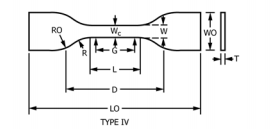
\includegraphics{Figs/PROBETA.PNG}}
    \caption{Dimensiones de la Probeta \citep{laureto}}
    \label{fig:probeta}
\end{figure}

\begin{table}[H]
\begin{center}
\begin{tabular}{c c c c}
\multicolumn{3}{c}{\textbf{Dimensiones Probeta}} \\
\toprule[0.6mm]
T & Espesor & 2  \\ 
W& Ancho de la sección estrecha &6 \\ 
L & Longitud  de la sección estrecha&35 \\ 
WO & Anchura total&20 \\ 
LO & Longitud total &115 \\ 
R & Radio de filete &14  \\
D & Distancia entre empuñaduras &70  \\
\bottomrule[0.6mm]
\end{tabular}
\caption{Valores Dimensiones \citep{laureto}}
\label{tabla:Medidas Probeta}
\end{center}
\end{table}

Para las condiciones a las cuales se va a desarrollar la prueba, se tiene en cuenta la siguiente \autoref{fig:prueba}


\begin{figure}[H]
    \centering
    \resizebox*{12 cm}{!}{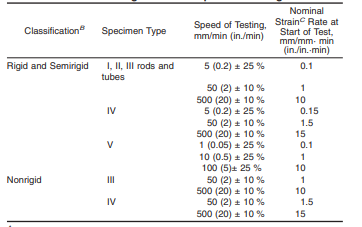
\includegraphics{Figs/pro_ta.PNG}}
    \caption{Designación Velocidades de Prueba \citep{laureto}}
    \label{fig:prueba}
\end{figure}

Se toma clasificación rígida o semirigida, probeta tipo IV, velocidad de prueba de 50 mm/min  COLOCAR LA MAQUINA CON LA QUE SE HACE Y LA TOLERANCIA, ya que se determina que es una velocidad promedio en todas las impresiones. Se utilizan las pruebas con probetas en diferentes orientaciones de construcción (0-45-90),proporcionando así los datos necesarios de resistencia requerida.\\

Con la implementación de cada una de estas características en el modelo STL ,se genera su respectivo G-code mediante el cual la impresora tendrá definido todo el modo de operación para la elaboración de la probeta.\\


\section{Norma ASTM D5379} \label{cortante}

Es una prueba estándar ,diseñada para medir las propiedades de corte de los materiales compuestos. El  procedimiento que se va a desarrollar se le conoce como corte de Iosipescu que se muestra en la \autoref{fig:cortante}.\\

Este método de prueba aplica una carga de compresión asimétrica de cuatro puntos a una muestra con muescas en V, lo que permite la aplicación de un solo esfuerzo cortante en el área de evaluación. Este método es ideal para probar una variedad de materiales laminados de CFRP, incluidos materiales de fibra unidireccionales, laminados ortogonalmente y discontinuos.\\

Este proceso permite realizar una Validación de las especificaciones,que confirman formalmente que sus productos y servicios cumplen con todos los estándares internos y externos de confianza. Garantizando una identificación previa de sus características, permitiendo mitigar el riesgo en el resultado final,\\

El ensayo se realiza bajo las mismas condiciones estándar que en el ensayo a tensión \acrshort{ASTM} D638, teniendo en cuenta las nuevas dimensiones mostradas en la \autoref{tabla:Medidascortante} COLOCAR LA MAQUINA CON LA QUE SE HACE Y LA TOLERANCIA . 

\begin{table}[H]
\begin{center}
\begin{tabular}{c c c c}
\multicolumn{3}{c}{\textbf{Dimensiones Probeta}} \\
\toprule[0.6mm]
T & Espesor & 5 \\ 
W& Distancia entre muescas& 1.4 \\ 
R & radio final muesca &1.3 \\ 
d2 & Anchura total&19 \\ 
L& Longitud total &76 \\ 
d1 & Profundidad de las muescas &3.8  \\

\bottomrule[0.6mm]
\end{tabular}
\caption{Valores Dimensiones \citep{laureto}}
\label{tabla:Medidascortante}
\end{center}
\end{table}


\begin{figure}[H]
    \centering
    \resizebox*{9 cm}{!}{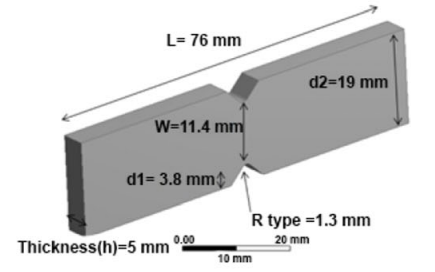
\includegraphics{Figs/probeta_cortante.PNG}}
    \caption{Probeta \acrshort{ASTM} D5379}
    \label{fig:cortante}
\end{figure}

Para los dos casos se manejara una cantidad total de 30 probetas, 15 para el ensayo a tensión \autoref{fig:probeta}, 5 por cada ángulo y 15 para el ensayo de cortante \autoref{fig:cortante}, 5 por cada ángulo. Se utiliza esta cantidad ya que de esta manera se brinda una estadística confiable en los resultados de las pruebas, determinando de manera idónea la resistencia final que posee la maquina construida, contra una de venta comercial.



\clearpage %poner esta linea al inicio de cada capitulo
\chapter{Discusión y Análisis de resultados}
\section{Resultados} \label{fotos}
\begin{center}
\textbf{Métodos de Verificación de Calidad}    
\end{center} 

\textbf{Cubo de Calibración}\\

Este dado de calibración es un modelo sencillo, rápido y fácil, El cual tiene como objetivo principal ajustar la precisión dimensional de la impresora modificando asi los pasos por mm que deberia tener el motor.\\

\textbf{Overhang test}\\

Como su nombre lo indica, este test es «todo en uno» para impresoras 3D contempla todo tipo de elementos: voladizos, puentes, encordado, extrusión, temperatura, tensión de la correa. Testea la impresora en todos los niveles lo que permite encontrar y ajustar los problemas que estén surgiendo en los modelos.\\

\textbf{ASTM D638}\\

Se realiza un ensayo a tensión a partir de una norma \acrshort{ASTM} la cual se presenta en la \autoref{norma}, Explicando todos sus requerimientos y desarrolló de la prueba.los resultados obtenidos son:

\\

\textbf{ASTM D5379}\\

Se realiza un ensayo cortante a partir de la norma \acrshort{ASTM} la cual se presenta en la \autoref{cortante}. En esta sección se muestran los requerimientos y desarrollo de la prueba. Los resultados obtenidos son:

\\


COLOCAR FOTOS DE LA MAQUINA PARA MOSTRAR QUE QUEDO IGUAL QUE EL DISEÑO

MOSTRAR LAS PROBETAS Y LOS ENSAYOS

MOSTRAR LA INTEGRACIÓN CON IOT QUE FUNCIONA MEDIANTE FOTOS O VIDEOS ALGUNA INTERFAZ

MOSTRAR LA PRESICION DE LOS CONTTROLES DE TEMPERATURA QUE SE IMPLEMENTARON




\section{Discusión }

INFORMACIÓN RELEVANTE PARA LA DISCUSIÓN 

huecos entre las capas depositadas, la variacion de capa a capa en su adición. la contracción durante el enfriamiento pueden causar en las propiedades mecanicas anisotropia(propiedad general de la materia segun cualidades como elasticidad, temperatura,conductividad, velocidad de propagación varian segun la direccion en la que estan siendo examinadas)\\

Es necesario destacar que parametros como orientación, espesor,temperatura, patron y densidad de relleno afectan o mejoran  de manera considerable las propiedades mecanicas del objeto en construcción. \\


las ventajas del PLA es que es de facil uso, prove un diseño confiable, se adhiere de manera sencilla y no le suceden deformaciones de gran magnitud. Para tener un estudio confiable de la resistencia del diseño que se entrega como resultado final, se implementa el estudio de los estandares ASTM, dirigido hacia las propiedades de tension y cortante en las probetas manufacturadas.\\

Las probetas se preparan con una densidad de 20 porciento y un patrón de relleno rectilinear,se utilizan 3 diferentes orientaciones 0 45 y 90, todo con el objetivo de evaluar el efecto en las propiedades mecánicas.

COLOCAR LA MAQUINA CON LA QUE SE REALIZA EL ENSAYO QUE CARAG SE LE APLICA Y CUAL ES LA TOLERANCIA DE LA MAQUINA. 

Se utiliza un filamento de 1.75 mm a una temperatura de .  


Escribir porque es mejor o peor dependioendo de los reusltados que se encontraron , inoveninetes tecnicos. bondades de esta respecto a otras y colocar que le falta a la maquina\\

COLOCAR AL FINAL LA PRESICION Y RESOLUCIOPN QUE SE VA A UTILZIAR PARA LA IMPRESIÓN 3D INCLUYENDO LA TOLERANCIA.\\

\addcontentsline{toc}{chapter}{Conclusiones}
\clearpage 
\chapter*{Conclusiones}

No es eficiente tener las dos manufacturas en una sola maquina DAR UNA EXPLICACION BIEN FUNDAMENTADA


MENCIONAR EL TRABAJO FUTURO QUE SE DEBE REALIZAR  para qeu le implementen LO QUE FALTA AL DISPOSITIVO para mejorarla.Colocar las limitaciones que tiene de integración final



\appendix

\chapter{Anexo I: QFD}
 \begin{figure}[H]
    \centering
    \resizebox*{14 cm}{!}{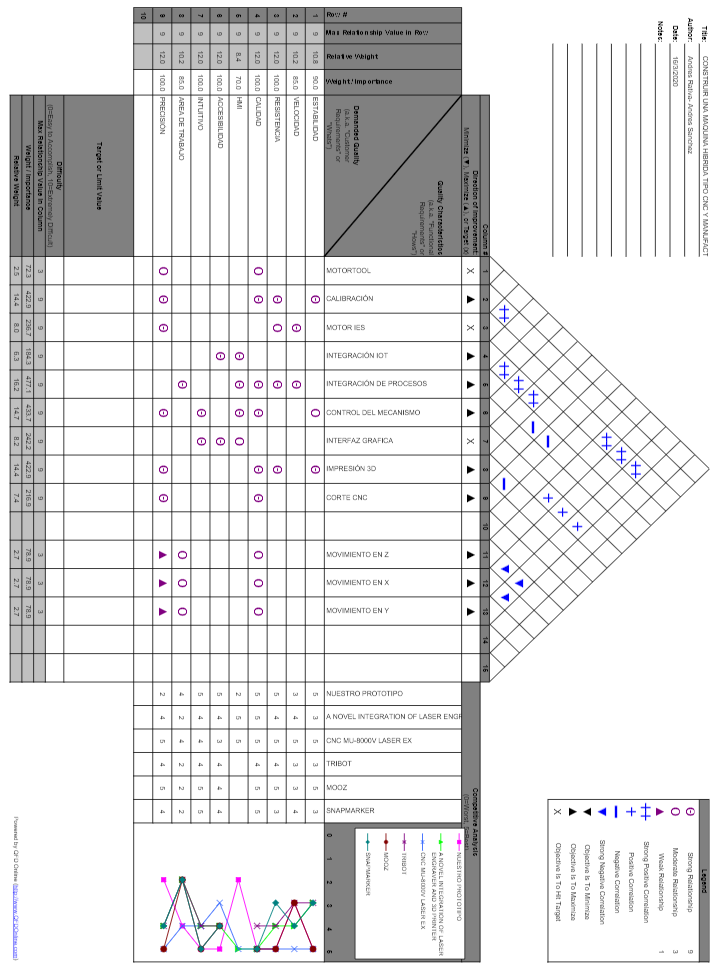
\includegraphics{Figs/QFD.PNG}}
    \caption{QFD}
    \label{fig:QFD}
\end{figure}

\chapter{Anexo II: BENCHMARK}

 \begin{figure}[H]
    \centering
    \resizebox*{15 cm}{!}{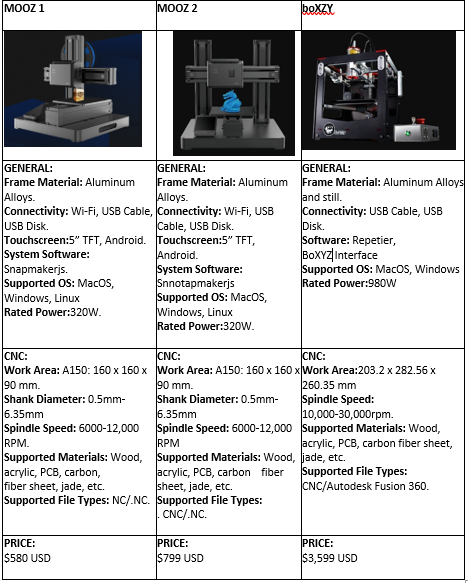
\includegraphics{Figs/benchamrk.PNG}}
    \caption{Benchmark}
    \label{fig:bench}
\end{figure}